\documentclass[usenames,dvipsnames]{beamer}
%-------------------------------------------------------
% THEME SETTINGS
%-------------------------------------------------------
\usetheme[progressstyle=movingCircCnt]{Feather}
\setbeamercolor{Feather}{fg=black!30,bg=black}
\setbeamercolor{structure}{fg=black}
\setbeamercolor{block body example}{bg=black!5!white}
\setbeamercolor{block title example}{fg=white,bg=black!40!white}


\usepackage{amsmath,amssymb,amsfonts}
\usepackage{cite}
\usepackage{multirow}
\usepackage{booktabs}
\usepackage{hhline}
\usepackage{multicol}
%\usepackage{showframe}

\usepackage{tikz}
%\usetikzlibrary{patterns}
\usetikzlibrary{patterns,arrows,decorations.pathmorphing,backgrounds,shadows,positioning,fit,shapes,matrix,calc,shapes.multipart,arrows.meta}
\usepackage[simplified]{pgf-umlcd}
\usepackage{xpatch} % Needed for patching pgf-umlcd
\usepackage{xparse} % Needed for patching pgf-umlcd
\usepackage{color,soul} % for \hl
\definecolor{dark-yellow}{RGB}{219, 212, 143}
\definecolor{dark-green}{RGB}{36,84,36}
\definecolor{my-gray}{gray}{0.85}
\sethlcolor{dark-yellow}



\usepackage{wrapfig}
\usepackage{listings}
\usepackage{adjustbox}
\usepackage{graphicx}
\usepackage{caption}
\usepackage{multirow}
\usepackage{subcaption}
\usepackage{stmaryrd}
\usepackage{hyperref}
\usepackage{float}
\usepackage{textcomp}
\usepackage{tikz-qtree,tikz-qtree-compat}

\newcommand*{\emphColorSlide}[1]{\textcolor{ForestGreen}{\textbf{#1}}}
\newcommand*{\emphSlide}[1]{\textcolor{ForestGreen}{\textbf{#1}}}

\newcommand*{\lowEmph}[1]{\textcolor{NavyBlue}{\textbf{#1}}}
\newcommand*{\subt}{\textcolor{NavyBlue}{\textbf{<:}}}
\newcommand*{\supt}{\textcolor{NavyBlue}{\textbf{:>}}}



\newcommand{\dataflow}{data-flow}
\newcommand{\Dataflow}{Data-flow}
\newcommand{\code}[1]{\texttt{\lstinline[basicstyle=\normalsize\ttfamily,identifierstyle={\normalsize},commentstyle={\normalsize\itshape},keywordstyle={\normalsize\bfseries},ndkeywordstyle={\normalsize},stringstyle={\normalsize\ttfamily},numberstyle={\normalsize}]!#1!}}
\newcommand{\CFG}{CFG}
\newcommand{\intraj}{\emphColorSlide{\textsc{Intra}J}}
\newcommand{\intrajs}{\emphColorSlide{\textsc{IntraJ}}}
\newcommand{\intracfgs}{\emphColorSlide{\textsc{IntraCFG}}}
\newcommand{\jastaddjintraflow}{\textsc{jastaddj-intraflow}}
\newcommand{\jji}{\code{JJI}}
\newcommand{\jastadd}{\textsc{JastAdd}}
\newcommand{\extendj}{\textsc{ExtendJ}}
\newcommand{\cG}{\mathcal{G}}
\newcommand{\cV}{\mathcal{V}}
\newcommand{\cE}{\rightarrowtail}
\newcommand{\cP}{\mathcal{P}}
\newcommand{\cM}{\mathcal{M}}


\newcommand{\mSyn}{\ensuremath{\uparrow}}
\newcommand{\mInh}{\ensuremath{\downarrow}}
\newcommand{\mHOA}{\ensuremath{\rightarrow}}
\newcommand{\mColl}{\ensuremath{\square}}
\newcommand{\mCirc}{\ensuremath{\circlearrowleft}}

\newcommand{\Abase}[1]{\textcolor{ATGsym}{\mbox{\umlcode{#1}}}}
\newcommand{\Asyn}[1]{\textcolor{ATGsym}{\mbox{\mSyn{}\umlcode{#1}}}}
\newcommand{\Ainh}[1]{\textcolor{ATGsym}{\mbox{\mInh{}\umlcode{#1}}}}
\newcommand{\Ahoa}[1]{\textcolor{ATGsym}{\mbox{\mHOA{}\umlcode{#1}}}}
\newcommand{\Acoll}[1]{\textcolor{ATGsym}{\mbox{\mColl{}\umlcode{#1}}}}
\newcommand{\Acirc}[1]{\textcolor{ATGsym}{\mbox{\mCirc{}\umlcode{#1}}}}

\newcommand{\umlcode}[1]{\textrm{#1}}  % Style of code used in UML fragments
\newcommand{\astnodestyle}{\ttfamily\color{magenta}}
\newcommand{\astnode}[1]{\texttt{\textcolor{magenta}{#1}}}  % Style used for AST node types

\newcommand{\ASTUnrestricted}{AST-unrestricted}
\newcommand{\ParentFirst}{Parent-First}

\newcommand{\project}[1]{\textsc{#1}}
\newcommand{\tool}[1]{\textsc{#1}}

% can't get fbox to work reliably in the UML code, and adjustbox and nested \tikz don't work at all
%\newcommand{\dfapi}{\textsf{\setlength{\fboxsep}{0pt}\fcolorbox{blue}{white}{df-api}}}
\newcommand{\dfapi}{\textbf{\textcolor{black}{[df-api]}}}
\newcommand{\nameapi}{\textbf{\textcolor{black}{[name-api]}}}

\newcommand{\frameworkname}{\textsc{Intra}CFG}
\newcommand{\intracfg}{\textsc{\frameworkname}}

\newcommand{\node}{\mathsf{n}}
\newcommand{\Null}{\mathtt{NULL}}
\newcommand{\Notnull}{\mathtt{NOTNULL}}
\newcommand{\gen}{\mathtt{gen}}
\renewcommand{\kill}{\mathtt{kill}}

\newcommand{\In}{\mathtt{in}}
\newcommand{\Out}{\mathtt{out}}
\newcommand{\Use}{\mathtt{use}}
\newcommand{\Def}{\mathtt{def}}
\newcommand{\tf}{f_t}
\newcommand{\mCi}[1]{ { \textcolor{black!30}{\tiny \pm\text{#1}}}}%Condifdence interval

\newcommand{\CR}[1]{\textbf{[}\textcolor{blue!60!black}{\textbf{CR:} #1}\textbf{]}}
\newcommand{\Ckw}[1]{\texttt{\textbf{#1}}}
\newcommand{\auxlabel}[1]{{\scriptsize{$\textrm{\texttt{#1}}$}}}
\newcommand{\auxlabeli}[2]{{\scriptsize{$\textrm{\texttt{#2}}_{#1}$}}}
\newcommand{\auxlabelbox}[1]{\tikz[baseline=-0.7ex] \node[rectangle, minimum width=0, thin, draw, rounded corners, fill=white, inner sep=2pt, outer sep=0pt] (N) {\auxlabel{#1}};}
\newcommand{\auxlabelboxhoa}[1]{\tikz[baseline=-0.7ex] \node[rectangle, dashed,minimum width=0, thin, draw, rounded corners, fill=white, inner sep=2pt, outer sep=0pt] (N) {\auxlabel{#1}};}

%\newcommand{\auxlabelboxi}[2]{\tikz \node[rectangle, minimum width=0, thin, draw, rounded corners, fill=white] {\auxlabeli{#1}{#2}};}

\newcommand{\Prod}{::=}
\newcommand{\terminal}[1]{\textcolor{green!50!black}{\textit{#1}}}
\newcommand{\vmetavar}[1]{\textcolor{cyan!30!black}{\textsf{\textbf{#1}}}}
\newcommand{\vcode}[1]{\textsf{\textcolor{green!35!black}{{#1}}}}
\newcommand{\vterminal}[1]{\vcode{#1}}
\newcommand{\nta}[1]{\ensuremath{\textit{#1}}}
\newcommand{\tuple}[1]{\ensuremath{\langle #1 \rangle}}
\newcommand{\nt}[1]{\ensuremath{\tuple{\hspace{-0.02cm}\nta{#1}\hspace{0.02cm}}}}
\newcommand{\VB}{\ |\ }
\newcommand{\Gcomment}[1]{\textrm{\textcolor{black!50!white}{({#1})}}}
\newcommand{\sem}[1]{\ensuremath{\llbracket #1 \rrbracket}}
%\newcommand{\semNPA}[1]{\ensuremath{\sem{#1}_{\textit{NPA}}}}
\newcommand{\semNPA}[1]{\ensuremath{\sem{#1}}}

\newcommand{\listingsfontsize}{\scriptsize}

\newcommand{\NAmark}{\multicolumn{1}{c}{\textcolor{black!40!white}{-}}}
\newcommand{\NAmarkR}{\multicolumn{1}{c|}{\textcolor{black!40!white}{-}}}
\newcommand{\Tcenter}[1]{\multicolumn{1}{c}{#1}}
\newcommand{\TcenterR}[1]{\multicolumn{1}{c|}{#1}}
\newcommand{\succarrow}{\tikz[baseline=-0.7ex] \draw[succarrow, thick, -{Stealth[scale=0.9, inset=0pt, angle'=45]}] (0,0) -- (0.3,0.0);}

\colorlet{hlgreen}{green}
\colorlet{hlorange}{orange}
\colorlet{hlgreenhalf}{green!50!white}
\colorlet{hlorangehalf}{orange!50!white}
\colorlet{npagrey}{gray!10!white}

\DeclareRobustCommand{\hlgreen}[1]{{\sethlcolor{hlgreenhalf}\hl{#1}}}
\DeclareRobustCommand{\hlorange}[1]{{\sethlcolor{hlorangehalf}\hl{#1}}}

\definecolor{ATGsym}{HTML}{206010}

\definecolor{SQ}{HTML}{0080ff}
\definecolor{JJI}{HTML}{ff0080}
\definecolor{IJnonH}{HTML}{004010}
\definecolor{IJH}{HTML}{00ff20}

\definecolor{succarrow}{HTML}{4e90e2}	% adapted from RunningExample.tex

\definecolor{lightblue}{HTML}{006699}		%#006699
\definecolor{lightgreen}{HTML}{669900}		%#669900
\lstdefinelanguage{JastAdd}{
  %keyword1&2&6
  morekeywords = [1]{class, extends, private, void,new},
  %keyword3
  morekeywords = [2]{this,null}, %JASTADD keywords
  %keyword4
  morekeywords = [3]{return}, %ASTnode typess
  %keyword5
  morekeywords = [4]{},
  keywordstyle = [1]\color{lightblue},
  keywordstyle = [2]\color{lightgreen},
%  keywordstyle = [1]\bfseries,
%  keywordstyle = [2]\bfseries,
  keywordstyle = [3]\astnodestyle,
  keywordstyle = [4]\color{orange},
  sensitive = true,
  morecomment = [l]{//},
  morecomment = [s]{/*}{*/},
  morecomment = [s]{/**}{*/},
  commentstyle = \color{gray},
  morestring = [b]",
  morestring = [b]',
  stringstyle = \color{purple}
}
\lstset{
  backgroundcolor =\color{npagrey},
  basicstyle=\listingsfontsize\ttfamily,
  identifierstyle={\listingsfontsize},
  commentstyle={\listingsfontsize\itshape},
  keywordstyle={\listingsfontsize\bfseries},
  ndkeywordstyle={\listingsfontsize},
  stringstyle={\listingsfontsize\ttfamily},
  frame={tb},
  breaklines=true,
  breakatwhitespace=true, %To avoid linebreaks between \code{} and comma.
  columns=[l]{fullflexible},
  numbers=none,
  numberstyle={\listingsfontsize},
  stepnumber=1,
  mathescape,
	escapeinside     = {!}{!}, %General escape does not seem to work in lstinline/GH.
}

\makeatletter
\pgfdeclareshape{topbottombox}{
  \inheritsavedanchors[from=rectangle]
  \inheritanchorborder[from=rectangle]
  \inheritanchor[from=rectangle]{center}
  \inheritanchor[from=rectangle]{base}
  \inheritanchor[from=rectangle]{north}
  \inheritanchor[from=rectangle]{north east}
  \inheritanchor[from=rectangle]{east}
  \inheritanchor[from=rectangle]{south east}
  \inheritanchor[from=rectangle]{south}
  \inheritanchor[from=rectangle]{south west}
  \inheritanchor[from=rectangle]{west}
  \inheritanchor[from=rectangle]{north west}
  \backgroundpath{
    %  store lower right in xa/ya and upper right in xb/yb
    \southwest \pgf@xa=\pgf@x \pgf@ya=\pgf@y
    \northeast \pgf@xb=\pgf@x \pgf@yb=\pgf@y
    \pgfpathmoveto{\pgfpoint{\pgf@xa}{\pgf@ya}}
    \pgfpathlineto{\pgfpoint{\pgf@xb}{\pgf@ya}}
    \pgfpathmoveto{\pgfpoint{\pgf@xa}{\pgf@yb}}
    \pgfpathlineto{\pgfpoint{\pgf@xb}{\pgf@yb}}
 }
}
\makeatother


% Patch UML package pgf-umlcd to be able to write abstract grammar as class name.
\ExplSyntaxOn
\NewDocumentCommand{\defineclassname}{m}
 {
  \tl_set:Nn \umlcdClassName { #1 }
  \tl_set_eq:NN \umlcdClassNameString \umlcdClassName
  \tl_replace_all:Nfn \umlcdClassName { \char_generate:nn { `_ } { 8 } } { \_\kern1pt }
 }
\cs_generate_variant:Nn \tl_replace_all:Nnn { Nf }
\ExplSyntaxOff
\xpatchcmd{\classAndInterfaceCommon}
 {\def\umlcdClassName}
 {\defineclassname}
 {}{}
\xpatchcmd{\endclass}
 {(\umlcdClassName)}
 {(\umlcdClassNameString)}
 {}{\ddt}
\xpatchcmd{\endinterface}
 {(\umlcdClassName)}
 {(\umlcdClassNameString)}
 {}{\ddt}
\xpatchcmd{\endabstractclass}
 {(\umlcdClassName)}
 {(\umlcdClassNameString)}
 {}{\ddt}
\xpatchcmd{\endobject}
 {(\umlcdClassName)}
 {(\umlcdClassNameString)}
 {}{\ddt}
\xpatchcmd{\endclassAndInterfaceCommon}
 {(\umlcdClassName)}
 {(\umlcdClassNameString)}
 {}{\ddt}
\xpatchcmd{\endclassAndInterfaceCommon}
 {(\umlcdClassName)}
 {(\umlcdClassNameString)}
 {}{\ddt}
\xpatchcmd{\endclassAndInterfaceCommon}
 {(\umlcdClassName)}
 {(\umlcdClassNameString)}
 {}{\ddt}

\newbool{ANON}
%\booltrue{ANON}
\boolfalse{ANON}
\newcommand{\anon}[2]
{\ifbool{ANON}{
   #1
}{
   #2
}}



\makeatletter
\renewcommand\@makefnmark{\hbox{\@textsuperscript{\usebeamercolor[fg]{footnote mark}\usebeamerfont*{footnote mark}[\@thefnmark]}}}
\renewcommand\@makefntext[1]{\@textsuperscript{\usebeamercolor[fg]{footnote mark}\usebeamerfont*{footnote mark}[\@thefnmark]}\usebeamerfont*{footnote} #1}
\makeatother

%Modify the Title display on frame
\makeatletter
\patchcmd\beamer@@tmpl@frametitle{\insertframetitle}{{\footnotesize \insertsection~\emphColorSlide{\insertsubsection}~\\} \textbf{\insertframetitle}}{}{}
\makeatother
%Add space to the footline
\makeatletter
\patchcmd{\beamer@calculateheadfoot}{\advance\footheight by 4pt}{\advance\footheight by 8pt}{}{}
\makeatother

%NO HEAD LINE
\makeatletter
\newenvironment{noheadline}{
	\setbeamertemplate{headline}[default] {}
	\setfootline
}{}
\makeatother

%Slide with  Section title
%\AtBeginSection[]{
%	\begin{noheadline}
%	\begin{frame}[noframenumbering]
%			\begin{center}
%				\large Chapter \thesection \\
%				\vspace*{1cm}
%				\centering {\usebeamerfont{title} \huge\textcolor{black}{\insertsectionhead}}
%				\vspace*{1cm}
%			\end{center}
%		\end{frame}
%	\end{noheadline}
%}


\newcommand{\setfootline}{
	\setbeamercolor{footline}{fg=white,bg=black}
	\setbeamertemplate{footline}{%
		\begin{beamercolorbox}[wd=1.0\paperwidth,left,ht=2.5ex,dp=1ex]{footline}
			\usebeamerfont{section in head/foot}%
			\hspace*{3.5ex}%
			\insertshortauthor\ |\
			\insertshorttitle
			\insertshortsubtitle
		\end{beamercolorbox}
	}
	\addtobeamertemplate{footline}{%
		\setlength\unitlength{1ex}%
		\begin{picture}(0,0)
		\put(125,3){\makebox(0,0)[bl]{
			
\includegraphics[scale=0.20]{img/scam.png}
	}}%
		\end{picture}%
	}{}
}






%-------------------------------------------------------
% INFORMATION IN THE TITLE PAGE
%-------------------------------------------------------

\subtitle[{\color{ForestGreen}\textbf{TAPL 2022}}]
{
	\footnotesize{TAPL 2022
}
}

\title[] % [] is optional - is placed on the bottom of the sidebar on every slide
{ % is placed on the title page
	\textsc{
	 Type Reconstruction}
}



\author[\textbf{Idriss Riouak}]
{ \emphSlide{Idriss Riouak}}

\institute[]
{\vspace{1cm}
	\textbf{Lund University}\\
	\textbf{Computer Science Department} \\
}

\date{\today}

\makeatletter
\newcommand\SoulColor{%
  \let\set@color\beamerorig@set@color
  \let\reset@color\beamerorig@reset@color}
\makeatother
\SoulColor

\begin{document}
\setfootline

%-------------------------------------------------------
% THE TITLEPAGE
%-------------------------------------------------------

{\1
\begin{frame}[plain,noframenumbering]
		\titlepage
	\end{frame}}

%-------------------------------------------------------
% BODY
%-------------------------------------------------------

\begin{frame}{Ch. 22 - Type reconstruction}
\hspace{-1cm}
\begin{minipage}[t]{0.4\textwidth}
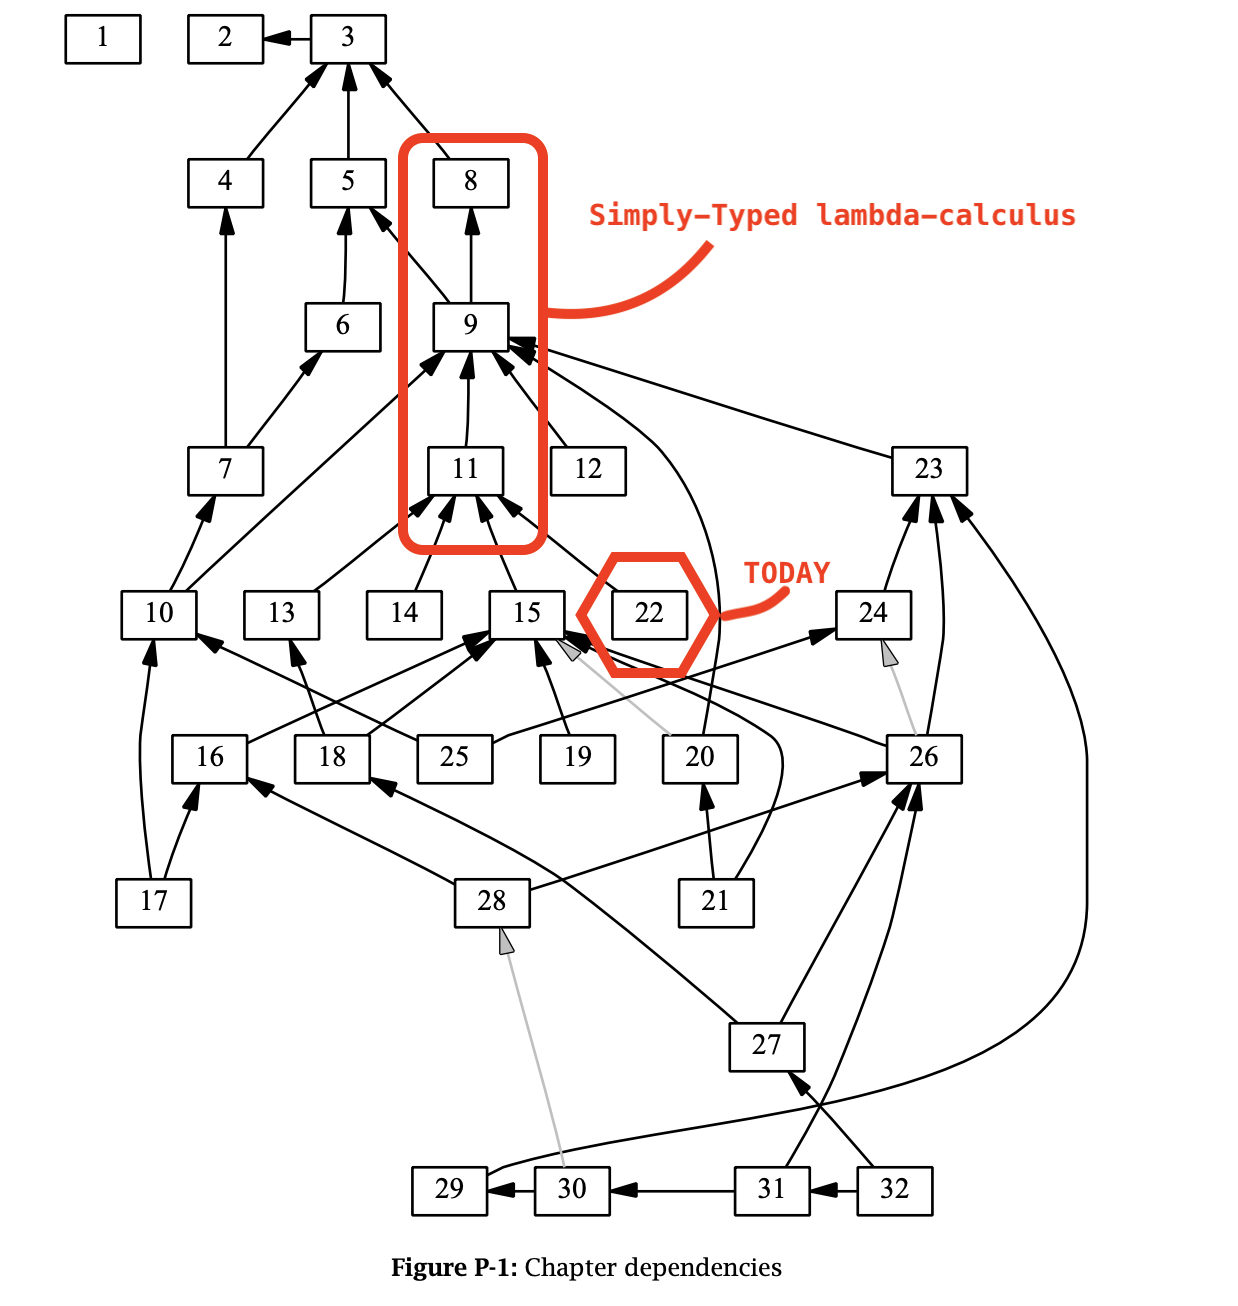
\includegraphics[scale=0.25]{img/depgraph}
\end{minipage}
\begin{minipage}[t]{0.4\textwidth}
\vspace{-5cm}
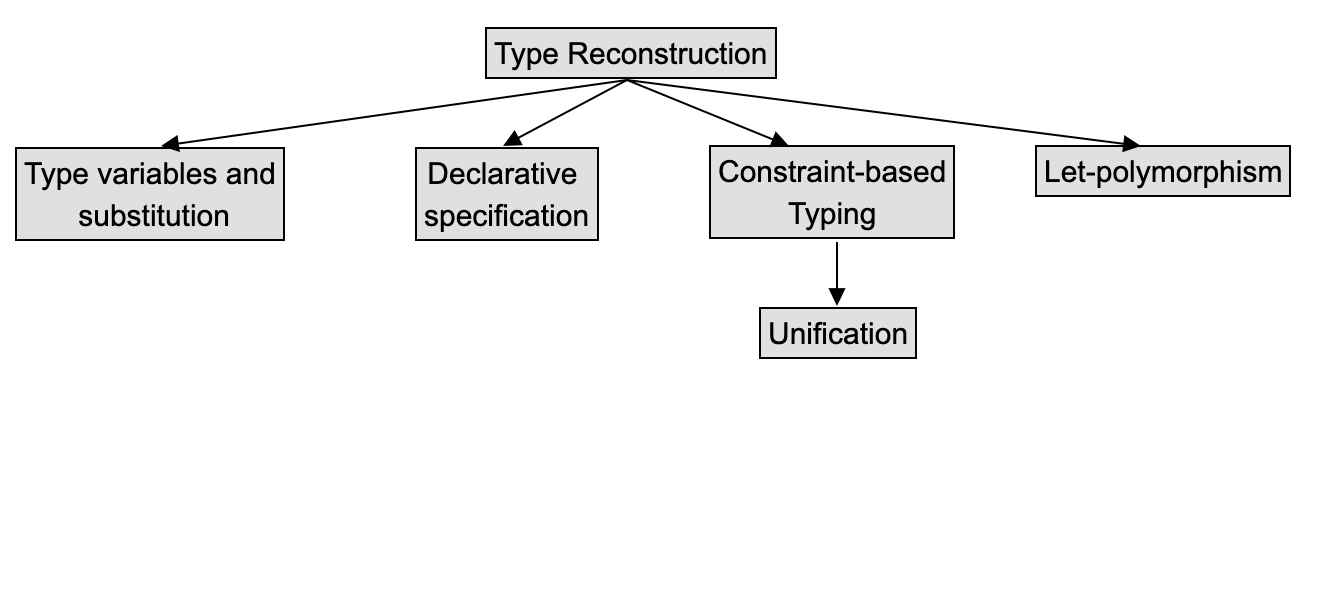
\includegraphics[scale=0.17]{img/1}
\end{minipage}
\end{frame}


\begin{frame}{Goal of today lecture}

\emphColorSlide{Type checking}: Given $\Gamma,t$ and $T$, \alert{check} whether $\Gamma \models t:T$.


\vspace{1cm}


\emphColorSlide{Type reconstruction}: Given $\Gamma$ and $t$, \alert{find} a type $T$ s.t. $\Gamma \models t:T$.
\end{frame}

\begin{frame}{Outline}
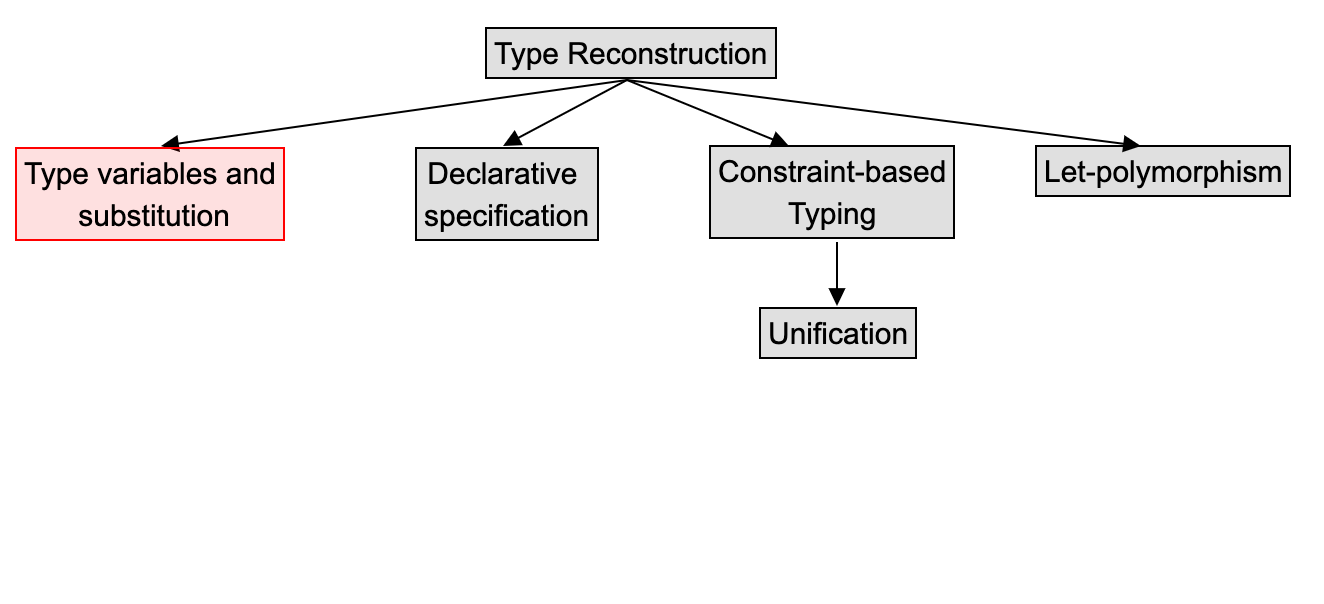
\includegraphics[scale=0.25]{img/2}
\end{frame}

\begin{frame}{Operations on type variables}
Let us consider the following term:
$$\lambda g:Y. \lambda a:X. g (g\ a)$$
\alert{it is not typable} as it stands.
\onslide<2->{
It is typable if we \emphColorSlide{substitute} $Y$ with $\mathtt{Nat} \rightarrow \mathtt{Nat}$ and $X$ with $\mathtt{Nat}$:
$$\lambda g:\mathtt{Nat} \rightarrow \mathtt{Nat}.  \lambda a:\mathtt{Nat}. g (g\ a)$$
}
\vspace*{-0.5cm}
\onslide<3->{
\begin{block}{Definition}
A type substitution is a finite mapping from type variables to types.
\end{block}}
\onslide<4->{
\begin{example}{}
The substitution $[Y \mapsto X \rightarrow X, X \mapsto \mathtt{Bool}]$ will map $X$ to $\mathtt{Bool}$, and $Y$ to $X \rightarrow X$, not $ \mathtt{Bool} \rightarrow  \mathtt{Bool}$
\end{example}
}
\end{frame}

\begin{frame}{Operation on type variables}
Application of a substitution $\sigma$ to a type:
\begin{align*}
\sigma(X) &= \begin{cases}
T & \text{if } (X \mapsto T) \in \sigma\\
X & \text{if } X \not\in dom(\sigma)
\end{cases}\\
\sigma(Nat) &= Nat\\
\sigma(Bool) &= Bool\\
\sigma(T_1 \rightarrow T_2) &= \sigma(T_1) \rightarrow \sigma(T_2)
\end{align*}


If $\sigma$ and $\gamma$ are substitutions:
$$\sigma \circ \gamma = \begin{cases}
X \mapsto \sigma(T)& \text{for each } (X \mapsto T)\in \gamma\\
X \mapsto T & \text{for each } (X \mapsto T) \in\sigma \wedge X \not\in dom(\gamma)
\end{cases} $$

TL;DR: $(\sigma \circ \gamma )S=\sigma(\gamma S)$
\end{frame}

\begin{frame}{Outline}
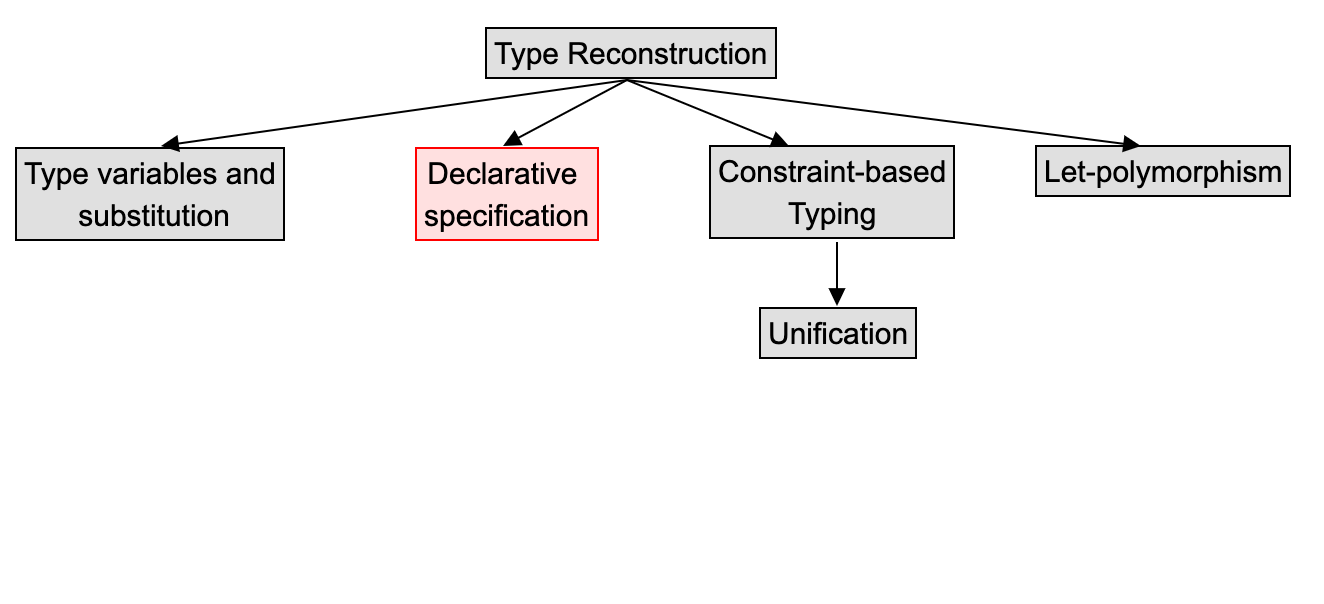
\includegraphics[scale=0.25]{img/3}
\end{frame}
\begin{frame}{Two interesting questions}
\begin{itemize}
\item ``Are \alert{all} substitution instances of $t$ well typed ?''\\
  i.e., $\forall \sigma. \sigma\Gamma \models \sigma t: T$ for some $T$ ?
\begin{example}
$\lambda g: X \rightarrow X.  \lambda a: X. g(g\ a)$
\end{example}
\item ``Is \emphColorSlide{some} substitution instance of $t$ well typed'' ? \\
  i.e., $\exists \sigma: \sigma\Gamma \models \sigma t: T$ for some $T$ ?
\begin{example}
$\lambda g: Y \rightarrow X.  \lambda a: X. g(g\ a)$
\end{example}

\end{itemize}
Looking for \emphColorSlide{valid instantiations} of type variables leads to the ideas of type \textit{reconstruction} (or type inference). The programmer (as in ML or Haskell) may leave out all type annotations.
\end{frame}


\begin{frame}{Type solution}
\begin{block}{Definition}
Let $\Gamma$ be a context and $t$ a term. A \emphColorSlide{solution} for $(\Gamma,t)$ is a pair $(\alert{\sigma},\emphColorSlide{T})$ s.t. $\alert{\sigma}\Gamma\models\alert{\sigma} t:\emphColorSlide{T}$.
\end{block}

\begin{example}
Let $\Gamma=g:X, a:Y$ and $t=g\ a.$ Then all the solutions for $(\Gamma,t)$ are:
\begin{itemize}
\item $([X \mapsto Y \rightarrow \mathtt{Nat}],\mathtt{Nat})$
\item $([X \mapsto Y \rightarrow  Z, Z \mapsto \mathtt{Nat}],Z)$
\item $([X \mapsto \mathtt{Nat} \rightarrow \mathtt{Nat}, Y \mapsto \mathtt{Nat}],\mathtt{Nat})$
\item $([X \mapsto Y \rightarrow Z],Z)$
\item $([X \mapsto Y \rightarrow \mathtt{Nat} \rightarrow \mathtt{Nat}],\mathtt{Nat})$
\end{itemize}
\end{example}


\end{frame}
\begin{frame}{Outline}
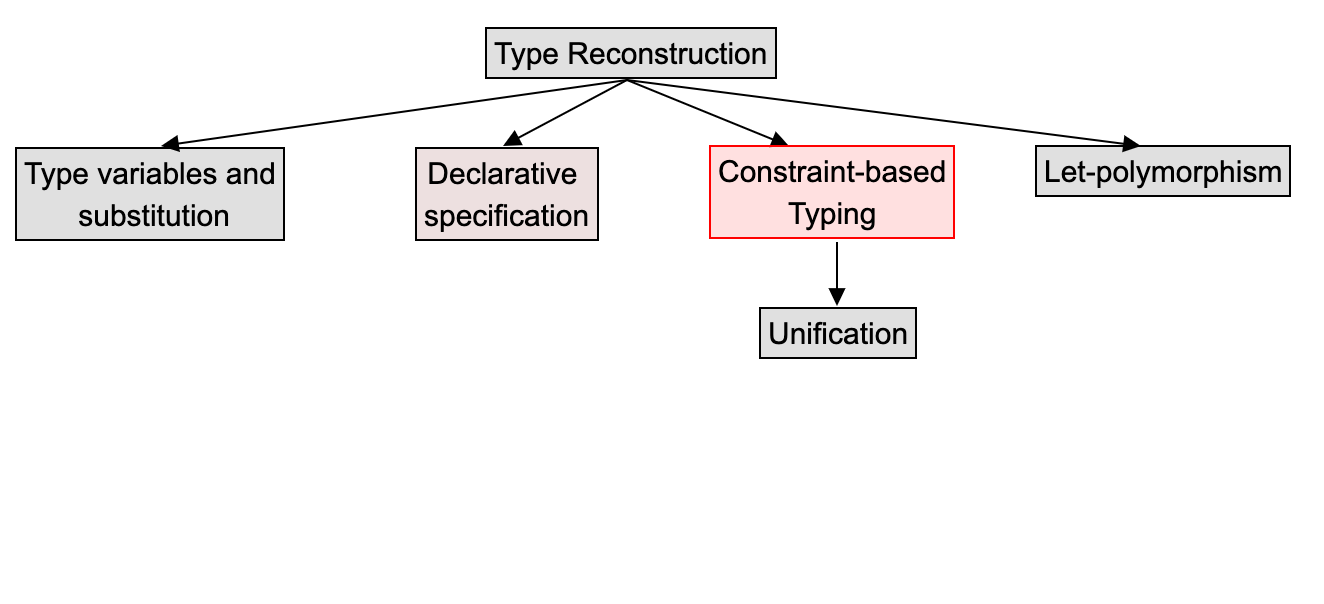
\includegraphics[scale=0.25]{img/4}
\end{frame}

\begin{frame}{Constraint-based typing}
\begin{block}{Definition}
\begin{itemize}
\item A \emphColorSlide{constraint set} C is a set of equations \{ $S_i = T_i^{i \in 1...n} $ \}.
\item A substitution $\sigma$ is said to \alert{unify} an equation $S=T$ if the substitution instances $\sigma S$ and $\sigma T$ are \emphColorSlide{identical}.
\item  We say that $\sigma$ unifies $C$ if it unifies \emphColorSlide{every equation} in C.
\end{itemize}
\end{block}

\begin{block}{Definition}
Suppose that $\Gamma \models t: S \mid_{\chi}C.$ A solution for $(\Gamma, t, S, C)$ is a pair $(\sigma, T)$ s.t. $\sigma$ satisfies $C$ and $\sigma S= T$.
\end{block}
 We read $\Gamma \models t :T \mid_\chi C$ as ``Term $t$ has type $T$ under assumptions $\Gamma$ whenever constraints $C$ are satisfied''
\end{frame}

\begin{frame}{Constraint typing rules}
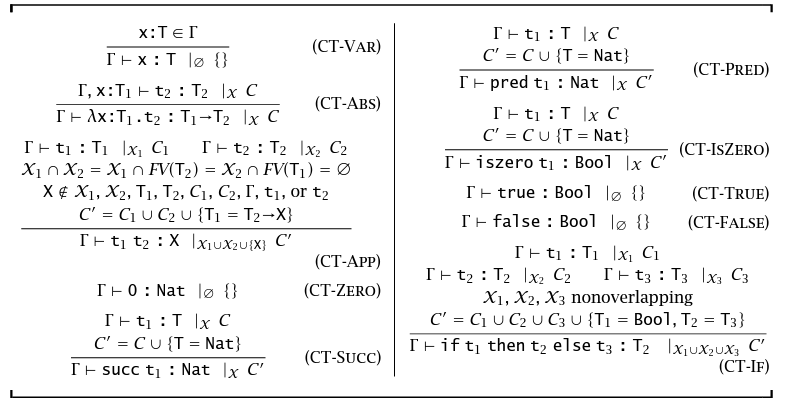
\includegraphics[scale=0.4]{img/rules}
\end{frame}

\begin{frame}{Declarative and Algorithmic specification}
Given a context $\Gamma$ and a term $t$, there are two ways of instantiating type variables in $\Gamma$ and $t$ to produce a valid typing:

\vspace{0.5cm}
\begin{enumerate}
\item[1)] \emphColorSlide{[Declarative]}: as the set of all solutions for $(\Gamma,t)$ in the sense of Definition 22.2.1
\item[2)] \emphColorSlide{[Algorithmic]}: via the constraint typing relation, by finding $S$ and $C$ such that $\Gamma \models t: S\mid C$ and then taking the set of solutions for $(\Gamma, t, S,C)$.
\end{enumerate}

\vspace{.5cm}
The two specification are equivalent.

\vspace{.5cm}
You can find the proof in the book :)

\end{frame}

\begin{frame}{Outline}
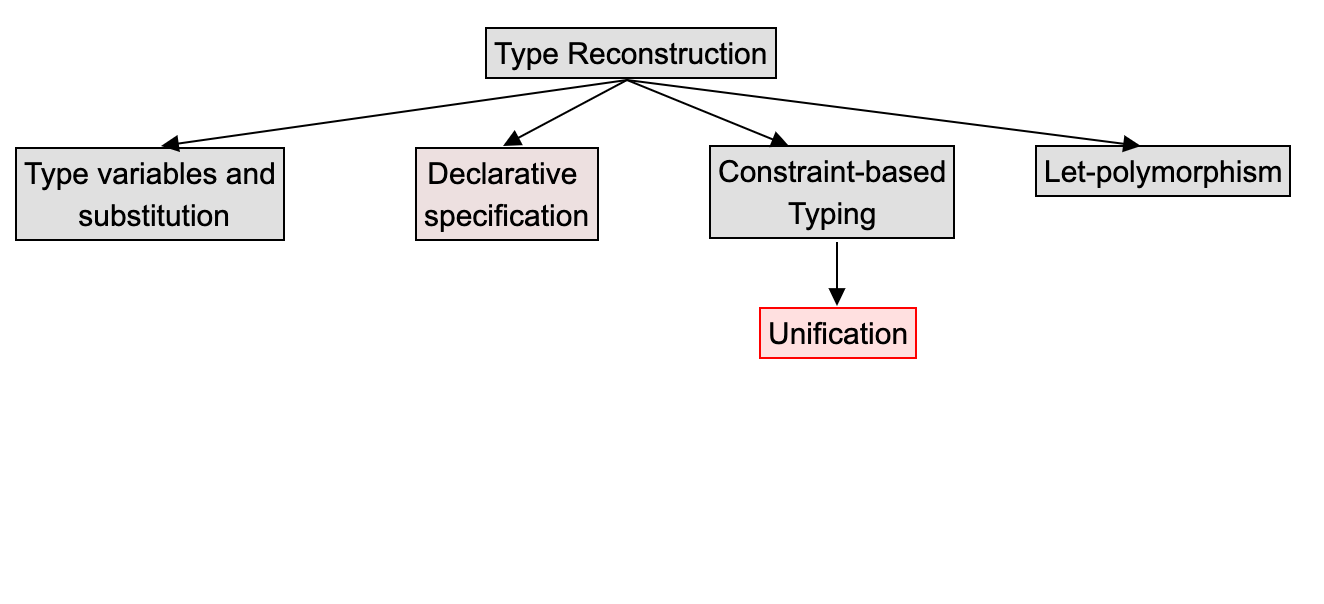
\includegraphics[scale=0.25]{img/5}
\end{frame}

\begin{frame}{Unification}
To compute solutions to constraint sets, we use the idea of unification\\
\vspace{0.5cm}
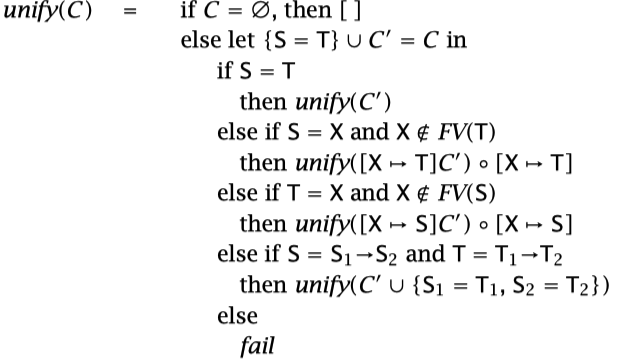
\includegraphics[scale=0.4]{img/unification}
\end{frame}

\begin{frame}{More about unification}
\begin{itemize}
\item We say that a substitution $\sigma$ is \emphColorSlide{less specific} than a substitution $\sigma'$, written $\sigma \sqsubseteq \sigma'$, if $\sigma' =  \gamma \circ \sigma$ for some substitution $\gamma$.
\item $\sigma$ is a \emphColorSlide{principal unifier} for a constraint set $C$ iff $$\forall \sigma' \in C: \sigma \sqsubseteq \sigma'.$$

\begin{theorem}
The algorithm `\emphColorSlide{unify}' always terminates, failing when given a non unifiable constraint set as input and otherwise returning a principal unifier.
\end{theorem}
\end{itemize}
\end{frame}

\begin{frame}{Outline}
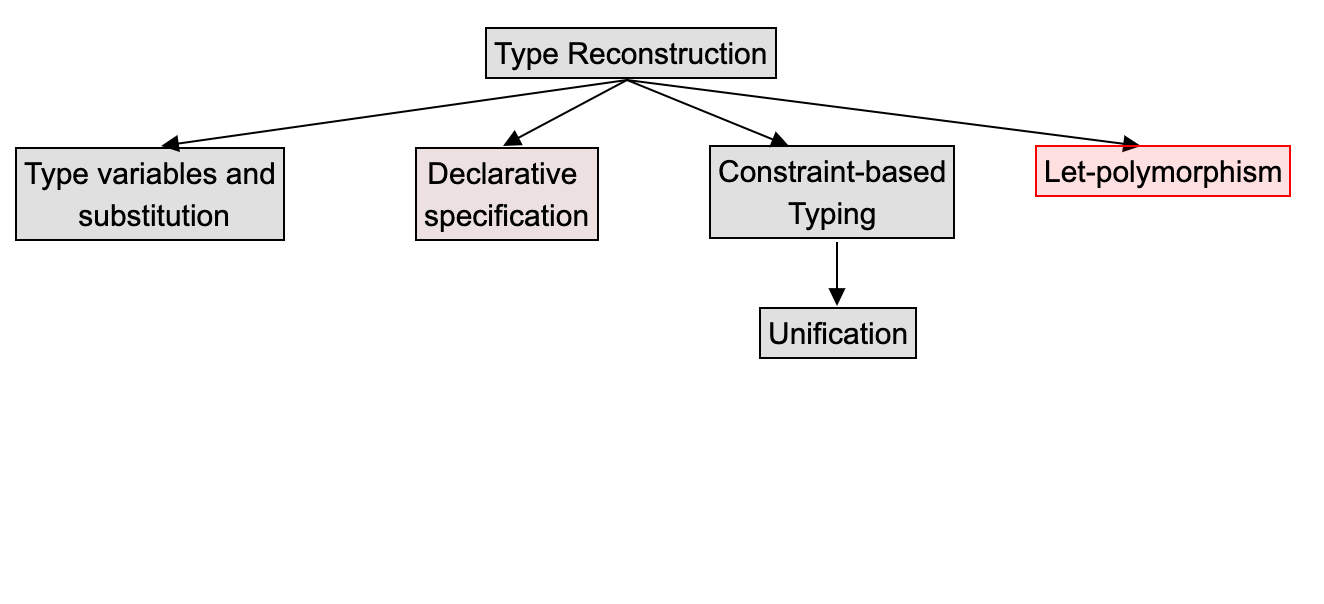
\includegraphics[scale=0.25]{img/6}
\end{frame}
\begin{frame}[fragile]{Let-polymorphism}
The term polymorphism refers to a range of language mechanisms that allow a single part of a program to be used with different types.

\begin{example}
\begin{lstlisting}[frame=none]
let f = \x.x in
let nat = f 1 in
let bool = f true in ...
\end{lstlisting}
\end{example}

\begin{itemize}
\item With the type reconstruction algorithms discussed previously, this program is not well-typed.
\item The type reconstruction algorithm shown before can be generalized to provide a simple form of polymorphism known as let-polymorphism.
\item More about polymorphism will be discussed next week.
\end{itemize}
\end{frame}

\begin{frame}{Let-polymorphism}
Old typing rule:
\begin{center}
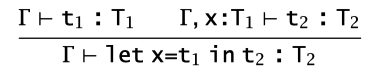
\includegraphics[scale=0.4]{img/old}
\end{center}

New  typing rule:
\begin{center}
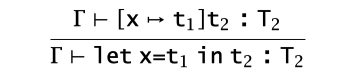
\includegraphics[scale=0.4]{img/new}
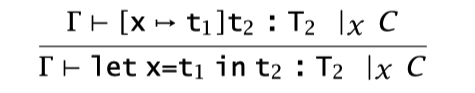
\includegraphics[scale=0.3]{img/newconstraint}
\end{center}
\onslide<2->{
What about `\texttt{let x = <garbage> in 5}' ?
}
\onslide<3->{
\begin{center}
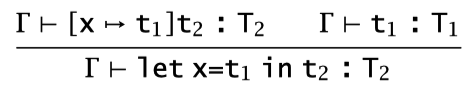
\includegraphics[scale=0.4]{img/newnew}
\end{center}
}

\end{frame}

%\begin{frame}{Algorithmic let-polymorphism}
%The type-checking of a term \code{let x = $\mathtt{t_1}$ in\ $\mathtt{t_2}$} in a context $\Gamma$ proceeds as follows:
%\begin{itemize}
%\item Calculate a type $S_1$ and a set $C_1$ of associated constraints for the right-hand side $t_1$.
%\item Obtain $t_1$'s principal type $T_1$
%\item If $X_1...X_n$ are the remaining variables in $T_1$, we write $\forall X_1...X_n.T_1 $ for the principal type scheme of $t_1$.
%\item Each time we encounter an occurrence of $x$ in $t_2$, we generate fresh $Y_1...Y_n$, yielding [$X_1\mapsto Y_1, ..., X_n \mapsto Y_n$ ]$T_1$.
%\end{itemize}
%
%\end{frame}

\begin{frame}{Essentially linear}
The algorithm is efficient ad in practice it appears ``\emphColorSlide{essentially linear}'' in the size of the input program. But the worst-case complexity is still \alert{exponential}.

\vspace{0.5cm}
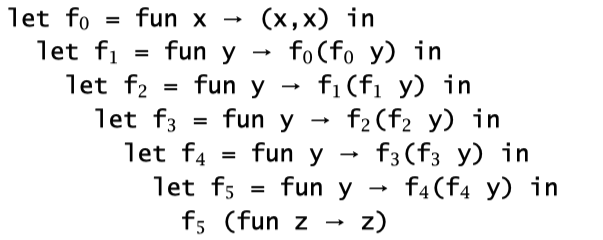
\includegraphics[scale=0.4]{img/expo}

\end{frame}

\begin{frame}{Conclusion}
\begin{center}
Type reconstruction algorithm \\ =\\ \emphColorSlide{Constraint generation} \\+\\\emphColorSlide{unification}.
\end{center}


\vspace{1cm}

\begin{center}
First introduction to\emphColorSlide{ polymorphism}
\end{center}

\end{frame}

%No page Numbering
\setbeamercolor{headline}{fg=white,bg=black}
\setbeamertemplate{headline}{
	\begin{beamercolorbox}[wd=1.0\paperwidth,left,ht=38pt,dp=1ex]{headline}
	\end{beamercolorbox}
	\vspace*{2.3pt}
	\color{black!30!white}\rule{\paperwidth}{2pt}
}


\end{document}